\documentclass[a4paper,10pt] {article}
\usepackage[spanish]{babel}
\usepackage[utf8]{inputenc}
\usepackage{caratula}
\usepackage{a4wide}
\usepackage{graphicx}

\begin{document}

\titulo{Trabajo Pr\'actico Nro. 2}
\fecha{08/05/2009}
\materia{Algoritmos y Estructuras de Datos III}
\grupo{}
\integrante{Dinota, Mat\'ias}{076/07}{matiasgd@gmail.com}
\integrante{Huel, Federico Ariel}{329/07}{federico.huel@gmail.com}
\integrante{Leveroni, Luciano}{360/07}{lucianolev@gmail.com}
\integrante{Mosteiro, Agust\'in}{125/07}{agustinmosteiro@gmail.com}

\maketitle

\bigskip
\section*{Aclaraci\'ones generales}

Antes de comenzar el an\'alisis de cada ejercicio, cabe mencionar lo siguiente:

\begin{itemize}
 \item La implementaci\'on de los 3 algoritmos se realizó en \textbf{lenguaje Java}, haciendo uso de las librer\'ias est\'andar del mismo.
 \item Para varios de los experimentos realizados se utiliz\'o un rango de n\'umeros acotado cuyo m\'aximo valor es $2^{31}-1$, ya que este es el valor m\'aximo del tipo de datos \textit{int}, utilizado para representar los n\'umeros naturales y enteros en las implementaciones propuestas.
 \item Para el c\'alculo de tiempo de los algoritmos se utiliz\'o la funci\'on \textbf{nanoTime()} de la clase System de Java.
 \item El c\'odigo fuente de los algoritmos aqui analizados se encuentran en los archivos \textit{Dengue.java} (Ej 1), \textit{...} (Ej 2) y \textit{...} (Ej 3).
 \item El c\'odigo fuente de los programas encargados de hacer uso de los algoritmos y necesarios para compilar las aplicaciones son:
 \begin{itemize}
    \item \underline{Ej 1:} MainDengue.java, Dengue.java e InstanciaDengue.java.
    \item \underline{Ej 2:} ...
    \item \underline{Ej 3:} ...
  \end{itemize}
 \item Para la lectura y escritura de los datos se utilizaron clases provistas por el lenguaje Java. No se har\'a referencia a estos algoritmos ya que no resultan de inter\'es para el trabajo aqui presentado.
 \item Al ejecutar cada programa sin argumentos se muestra una leyenda explicando su modo de uso.
 \item Los gr\'aficos se realizaron con \textbf{GNUPlot}. En los casos considerados pertinentes, se utiliz\'o una escala logar\'itmica con el fin de poder visualizar mejor los resultados.
\end{itemize}

\begin{center}
\section*{Ejercicio 1: Dengue}
\end{center}

\bigskip
\section*{Introducci\'on}

La idea de este ejercicio es intentar demostrar de manera emp\'irica la
conjetura de Goldbach. Esta misma predica que todo n\'umero par positivo mayor
que dos se puede escribir como la suma de dos n\'umeros primos. Con este
objetivo se procedi\'o a la implementaci\'on de un algoritmo iterativo que, dado
un n\'umero par mayor que dos, retorna dos n\'umeros primos que satisfacen dicha
conjetura.

En principio, se probaron distintos casos aleatorios para encontrar un patr\'on
com\'un. A partir de esto, se realiz\'o la siguiente conjetura: ``Sea $p$ el mayor primo comprendido en el rango $3..n-2$ entonces $p$ y $n-p$ son dos n\'umeros primos cuya suma es $n$''. De ser cierta esta conjetura, bastar\'ia con hallar el primo m\'as cercano a $n-2$ para obtener, mediante operaciones ba\'asicas, el resultado esperado. Sin embargo, al poco tiempo se encontr\'o un contraejemplo ($128 = 119 + 9$, pero 9 no es primo) que falseaba la conjetura. A pesar de esto, la idea sirvi\'o para encontrar una soluci\'on al problema. En la secci\'on siguiente veremos el algoritmo en cuesti\'on.

\section*{Algoritmo}

A continuaci\'on se encuentra el pseudoc\'odigo relativo al algoritmo propuesto
que resuelve el problema, seguido de una breve explicaci\'on acerca del
funcionamiento del mismo.

\begin{verbatim}
maxMMParcial[0..zonas][0..litros]

para j desde 0 hasta litros
  maxMMParcial[0][j] = 0

para i desde 0 hasta zonas
  para j desde 0 hasta litros
    max_parcial = M[i-1,j]
    k = 1
    mientras k <= j
      max_parcial = maximo(max_parcial, M[i-1,j-k] + MM[i][k])
    maxMMParcial[i][j] = max_parcial

litrosPorZona[0..zonas-1]
litrosRestantes = litros
j = litrosRestantes
para i desde zonas hasta 1
  mientras j >= 0 y (maxMMParcial[i][litrosRestantes] - MM[i-1][litrosRestantes - j]) != maxMMParcial[i-1][j]
    j = j - 1
  litrosPorZona[i-1] = litrosRestantes - j
  litrosRestantes = j

guardar en Tp2Ej1.out la linea "maxMMParcial[zonas][litros]"
para i desde 0 hasta zonas-1
  guardar en Tp2Ej1.out el valor "litrosPorZona[i]"

\end{verbatim}

% En primer lugar, se encuentr\'a la definici\'on de la funci\'on \textit{esPrimo}
% que, tal como su nombre indica, retorna \textit{true} en caso de que el n\'umero
% pasado como par\'amentro sea un n\'umero primo y \textit{false} en caso
% contrario. El algoritmo en cuesti\'on consiste en un m\'etodo simple pero
% efectivo: En primer lugar, hay 2 casos base, el primero retorna \textit{true} en caso de
% tratarse del n\'umero 2 y el segundo evalua si el numero es par (divisible por
% 2), retornando \textit{false} en este caso, ya que todo numero par mayor que 2
% no es primo. Luego, el ciclo principal evalua si el par\'ametro $n$ es divisible
% por alg\'un n\'umero impar $i$ con $3 \leq i \leq \sqrt{n}$, retornando
% \textit{false} en tal caso. La correctitud de tal procedimiento se desprende
% directamente del teorema que predica que si $n$ es un n\'umero primo entonces
% existe al menos un divisor d tal que $2 \leq d < \sqrt{n}$.
% 
% Con respecto al algoritmo relativo al problema en s\'i, la idea consiste en
% recorrer todos los n\'umeros impares comprendidos entre $3$ y $n-3$ de a pares
% cuya suma equivalgan a $n$. Los pares $i, n - i$ satisfacen trivialmente esta condici\'on, ya que $i + (n-i) = n$. Del mismo modo, es f\'acil ver que para generar todos los n\'umeros del rango mencionado, basta con variar i tal que $3 \le i \le n/2$. De esta forma se ve claramente que esPrimo(i) comprende el rango $3..n/2$, y $esPrimo(n-i)$ el rango $n/2..n-3$. De este modo, cuando se satisface que $esPrimo(i) \& esPrimo(n-i) == true$ se puede afirmar que se ha encontrado el par de n\'umeros que cumplen con la conjetura: dos n\'umeros primos cuya suma es $n$. En caso de que no hallar dicha tupla dentro del rango propuesto, se puede concluir que la conjetura de Goldbach era falsa, retornando la tupla (0,0) en este caso.  

\section*{Correctitud}

En esta secci\'on se analizar\'a en detalle la validez del algoritmo propuesto anteriormente. En primer lugar, se mostrar\'a c\'omo aplica el principio de optimalidad al problema dado. En segundo lugar, se demostrar\'a la correctitud del algoritmo expres\'andolo de forma recursiva para facilitar dicha demostraci\'on. Finalmente, se mostrar\'a que la forma recursiva del algoritmo y la versi\'on presentada en anteriores secciones son equivalentes en t\'erminos de correctitud por lo que quedar\'a demostrada la correctitud del algoritmo propuesto.
  
\subsection*{Principio de optimalidad}

Demostraremos por qu\'e vale el principio de optimilidad en este problema por el absurdo.

Sean $n$ y $l$ la cantidad de zonas y litros disponibles respectivamente y que las zonas se numeran de $1$ a $n$. Suponemos que la cantidad de mosquitos muertos con $l$ litros hasta la zona $n$ es \'optima y llamaremos $P$ a dicha cantidad. Sea $k$ la cantidad de litros usados en la zona $n$, suponemos que hasta la zona $n-1$ usando $l-k$ litros la cantidad de mosquitos muertos ($Q$) no es \'optima y se intenta llegar a un absurdo.

Si hasta la zona $n-1$ la cantidad de mosquitos muertos no es \'optima (para $l-k$ litros), existe otra forma de distribuir los $l-k$ litros entre las zonas $1$ a $n-1$ que hace que la nueva cantidad, a la que llamaremos $R$, sea \'optima (es decir, $R > Q$). Entonces tenemos que

$R + cantMM(n,k) > Q + cantMM(n,k) = P \Rightarrow R + cantMM(n,k) > P$

Esto es un absurdo ya que supusimos que $P$ era la cantidad \'optima. Este absurdo surge de suponer que la cantidad de mosquitos muertos hasta la zona $n-1$ con $l-k$ litros no era \'optima. Entonces queda demostrado que vale el principio de optimalidad para el problema planteado.

\subsection*{Demostraci\'on de correctitud}

A partir de la idea presentada en la secci\'on anterior se puede plantear la siguiente funci\'on recursiva para resolver el problema.

$\\ f(1,l) = max_{1 \leq j \leq l} (MM[1][j]) \\
 f(i,l) = max_{0 \leq k \leq l} (f(i-1, l-k) + MM[i][k]) \;\;\;\; $ si $i > 1
$ \\

Siendo $MM[i][j]$ la matriz que contiene la cantidad de mosquitos muertos por litro, de cada zona. La soluci\'on al problema ser\'ia $f(n,l)$ con $n$ la cantidad de zonas y $l$ la cantidad de litros disponibles.

Para demostrar que la funci\'on presentada es correcta utilizaremos inducci\'on en la cantidad de zonas manteniendo la cantidad $l$ de litros fija. Es decir, queremos probar la siguiente proposición. \\

P(n): $f(n, i)$ es la cantidad máxima de mosquitos muertos hasta la zona $n$ con $i$ litros. ($0 \leq i \leq l$) \\

\textbf{Caso Base ($P(1)$)}

$f(1,i) = max_{1 \leq j \leq i} (MM[1][j]) \;\;\;\; $ con $i \leq 1$

Entonces, como se puede notar, $f(1,i)$ es trivialmente la cantidad máxima de mosquitos muertos de la primera zona con $i$ litros. \\

\textbf{Paso inductivo ($P(n) \Rightarrow P(n+1)$)}

Supongo que $f(n,i)$ es la máxima cantidad de mosquitos muertos hasta la zona $n$ con $i$ litros ($0 \leq i \leq l$) y demuestro que $f(n+1,i)$ es la cantidad máxima hasta la zona $n+1$.
Como $n+1 > 1$ tenemos que \\

$f(n+1,i) = max_{0 \leq k \leq i} (f(n, i-k) + MM[n+1][k])$ \\

Como $i - k \leq l$ para cualquier $k \leq i$ puedo aplicar la hipótesis inductiva, es decir, $f(n,i-k)$ es la máxima cantidad hasta la zona $n$ con $i-k$ litros. Entonces con $max_{0 \leq k \leq i} (f(n, i-k) + MM[n+1][k])$ obtengo la máxima cantidad de mosquitos muertos hasta la zona $n+1$ con $i$ litros pues $f(n,i-k)$ es máxima y se calcula el máximo para todas las cantidades $k$ de litros posibles para dicha zona. Entonces, como vale $P(1)$ y $P(n) \Rightarrow P(n+1)$ por principio de inducci\'on queda demostrada la proposici\'on.

\subsection*{Equivalencia entre la función recursiva y el algoritmo presentado}


\section*{Complejidad}

A continuaci\'on se analizara la complejidad de peor caso sobre los modelos
uniforme y logaritmico.

Nota: En el siguiente an\'alisis se hara referencia a funciones propias de la implementaci\'on de los algoritmos. Puede ver el c\'odigo fuente del mismo en la secci\'on \textit{Anexos}.

\subsection*{Modelo Uniforme:}

En este modelo el an\'alisis no esta centrado en el tama\~{n}o de los operandos
por lo que el tiempo de ejecuci\'on de cada operaci\'on se considera constante.

En la funci\'on \textit{esPrimo} todas las operaciones y asignaciones utilizadas se
logran en tiempo constante por lo mencinado anteriormente, de esta manera la
complejidad de esta funci\'on depende del ciclo que contiene. Como itera sobre
\textit{i} entre 3 (valor de inicializaci\'on) y $\sqrt{n}+1$, y ademas en cada
vuelta del ciclo la variable es aumentada en 2, claramente se aprecia que en el
peor caso (es decir que nunca se cumpla la condici\'on n mod i = 0) el ciclo se
recorre aproximadamente $\sqrt{n}/2$ veces. De esta manera concluimos que $T(n)
\in O(\sqrt{n})$.

En cuanto a la complejidad de las operaciones y asignaciones realizadas en la
funci\'on \textit{encontrarPrimos} el caso es el mismo al de \textit{esPrimo} debido al modelo de
computo. La unica operaci\'on dentro del pseudocodigo de encontrarPrimos de
complejidad superior a constante es la analizada anteriormente y dicha operacion se
encuentra dentro del \'unico ciclo de la funci\'on por lo que concentraremos el
an\'alisis de complejidad aqui. En este caso iteramos sobre el mismo valor de
inicio pero el limite del ciclo esta dado por $n/2$. Tambien aqui la variable
\textit{i} es aumentada en 2 en cada iteraci\'on lo que determina que en el peor
caso se iterar\'a aproximada mente $(n/2)/2 = n/4$ veces. Como dentro del ciclo
se llama a esPrimo (complejidad $\sqrt{n}$) la complejidad final de la funci\'on
encontrarPrimos es $T(n) \in O(n*\sqrt{n})$.

\subsection*{Modelo Logar\'itmico:}

En este modelo de computo si nos concentraremos en el tama\~{n}o de la entrada y
el costo de las operaciones en funci\'on de la cantidad de bits de sus
operandos.

En la funci\'on \textit{esPrimo} se puede apreciar que las operaci\'ones que mayor
complejidad conllevan son $\sqrt{n}$ y $n$ mod $i$. Como ambas son llamadas
dentro del \'unico ciclo de la funci\'on, la complejidad estar\'a determinada
por dicho ciclo.

Entonces tenemos 

$$ T(n) = \sum_{i=3,i\,mod\,2=1}^{\sqrt{n}}
[\log(\sqrt{n}+1)+\log(n)^{2}+\log(n)^{2}+\log(n\,mod\,i)+\log(i)] $$
$$\leq \sum_{i=1}^{\sqrt{n}} [\log(n)+2\log(n)^{2}+\log(n)+\log(n)] $$
$$= \sqrt{n}(3\log(n)+2\log(n)^{2}) \Longrightarrow T(n) \in O(\sqrt{n}*\log(n)^{2})$$

\bigskip

Con respecto a la funci\'on \textit{encontrarPrimos} sucede lo mismo con respecto a que
las operaciones de mayor complejidad son realizadas dentro del ciclo por lo que
en este caso la complejidad total de la funci\'on tambi\'en estar\'a determinada
por dicho ciclo.

La funci\'on de complejidad es 
$$ T(n) = \sum_{i=3,i\,mod\,2=1}^{n/2}
[\log(i)+\sqrt{i}*\log(i)^{2}+\sqrt{n-i}*\log(n-i)^{2}+\log(n)+\log(n)+\log(i)] $$
$$ \leq \sum_{i=1}^{n} [\log(n)+\sqrt{n}*\log(n)^{2}+\sqrt{n}*\log(n)^{2}+\log(n)+\log(n)+\log(n)] $$
$$ = n*(4*\log(n)+2*\sqrt{n}\*log(n)^{2}) \Longrightarrow T(n) \in O(n^{3/2}*\log(n)^{2}) $$

\bigskip

Por \'ultimo analizaremos tambi\'en la complejidad en funci\'on del tama\~{n}o
de la entrada para los dos modelos de c\'omputo vistos. Como la funci\'on
encontrarPrimos toma unicamente un natural \textit{n}, si llamamos \textit{t} al
tama\~{n}o de entrada tenemos que $t = \log(n) \Longrightarrow 2^{t} = n$. De
esta manera, reemplazando $n$ en las complejidades calculadas previamente
obtendremos el costo de los dos algoritmos.

\begin{itemize}
\item Modelo Uniforme: 
$$T(n) \in O(n\sqrt{n}) = O(n^{3/2}) \Longrightarrow T(t) = O((2^{t})^{3/2}) =
O(2^{3t/2})$$
\item Modelo Logar\'itmico: 
$$T(n) \in O(n^{3/2}\log(n)^{2}) \Longrightarrow T(t) =
O((2^{t})^{3/2}(\log(2^{t}))^{2}) = O((2^{3t/2}t^{2})$$
\end{itemize}

\section*{An\'alisis de resultados}

%TODO: matrices generadas aleatoriamente

Con el fin de analizar la complejidad del algoritmo propuesto se realizaron algunas pruebas. Estos experimentos están orientados a estudiar el tiempo de ejecución del mismo en relaci\'on a los datos de entrada, comparando el costo real del algoritmo junto con su complejidad teórica calculada. Debido a que el algoritmo en cuestión depende de dos parámetros de entrada, se realizaron pruebas separadas para cada uno de los parámetros. Las primeras dos pruebas analizan el costo de lo que anteriormente denominamos \textit{fumigación} en base a la cantidad de zonas en primer término y en segundo lugar a la cantidad de litros. La tercer y última prueba mostrará el tiempo de cálculo de los litros empleados por cada zona.|

En primer lugar, se hicieron cálculos en utilizando como variable la cantidad de zonas a fumigar, fijando en $10$ los litros disponibles. El rango de zonas analizados es desde $1$ hasta $10000$ zonas, de a intervalos de tamaño $10$. La elección de estos valores fue producto del análisis de 2 cuestiones importantes: que números permitirían tomar muestras utiles para la realización de los gráficos y cual era la máxima cantidad de datos que nuestra aplicación podría manejar, acotada por el tiempo disponible para realizar las pruebas y las limitacion propias de la máquina en cuestión. Empiricamente, se comprobó que dicho rango de zonas permitía correr la aplicación en un tiempo razonable y al mismo tiempo proveer datos interesantes para el análisis en cuestión. Del mismo modo, fijar en 10 los litros aseguró que sea la cantidad de zonas el parámetro ponderante en el cálculo de tiempo de ejecución.

La segunda prueba resulta muy similar a la anterior en cuanto al rango de valores utilizados. La diferencia radica en que ahora el parámetro fijado es la cantidad de zonas, variando los litros en el rango $1$ hasta $10000$, de a intervalos de tamaño $10$ (al igual que en la prueba anterior).

Por último, la última prueba consistió en comparar la compledijidad teórica del algortimo que calcula los litros utilizados para fumigar cada zona que maximizan la cantidad de mosquitos muertos. Para esto, 


\begin{verbatim}
Prueba 1
--------
mientras i <= 2^31-4
  T = tiempo que tarda la operacion encontrarPrimos(i) en microsegundos
  i = i + 10000 + numero aleatorio par entre 0 y 10000
  guardar en Ej1-Complejidad.txt la linea "i T"
\end{verbatim}

La segunda prueba tiene como objetivo mostrar que la cantidad de operaciones que realiza el algoritmo es significativa menor que la cota teorica propuestas, a\'un en los peores casos. Con este fin, se cre\'o una aplicaci\'on que obtiene los m\'aximos de la primer componente de la tupla soluci\'on (n\'umero primo mas chico) para 20 ejecuciones del algoritmo. Al igual que en la primer prueba, se opt\'o por un enfoque aleatorio, tomando muestras de n\'meros a intervalos aleatorios entre $10^{5}$ y $2*10^{5}$.

\begin{verbatim}
Prueba 2
--------
para j desde 0 hasta 20
  peor_caso_primo1 = 0
  mientras i <= 2^31-4
    <primo1, primo2> = encontrarPrimos(i)

    si primo1 > peor_caso_primo1
      peor_caso = i
      peor_caso_primo1 = primo1
      peor_caso_primo2 = primo2

    i = i + 100000 + numero aleatorio par entre 0 y 100000

  guardar en Ej1-MayoresPrimos.txt la linea "peor_caso peor_caso_primo1 peor_caso_primo2"
\end{verbatim}

Por \'ultimo, con el fin de observar m\'as en detalle el comportamiento del algoritmo se decidi\'o extraer los peores casos de la Prueba 1 y estudiarlos en profundidad (Prueba 3). Para realizar esta tarea, se implement\'o una sencilla aplicaci\'on (ver pseudoc\'odigo debajo) que toma alrededor de 200 secuencias consecutivas de 1000 n\'umeros aleatorios comprendidas entre $4$ y $2^{31}-4$ utilizando el mismo criterio que en el caso anterior. Luego, obtiene el m\'aximo tiempo de ejecuci\'on entre todos los n\'umeros de cada secuencia. 

\begin{verbatim}
Prueba 3
--------
j = 1
mientras i <= 2^31-4
  maximo_tiempo = 0
  T = tiempo que tarda la operacion encontrarPrimos(i) en microsegundos

  si T > maximo_tiempo
    maximo_tiempo = T
    peor_caso = i

  si j = 1000
    guardar en Ej1-Peorescasos.txt la linea "peor_caso maximo_tiempo"
  
  j = j + 1
  i = i + 10000 + numero aleatorio par entre 0 y 10000
\end{verbatim}

A continuaci\'on se presentan los resultados relativos a la primera aplicaci\'on (Prueba 1).

% \begin{center}
%  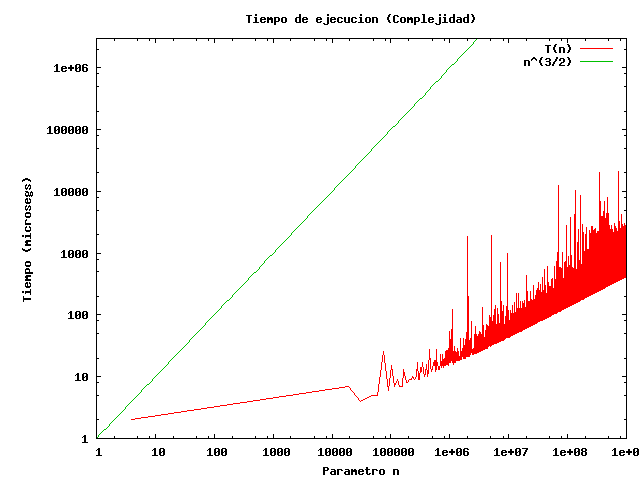
\includegraphics[width=0.7\textwidth]{Plots/Ej1-Complejidad.png}
% \begin{center}
% Figura 1.1
% \end{center}
% \end{center}

Este gr\'afico muestra la comparaci\'on entre las mediciones de tiempo de la primera prueba realizada y la complejidad te\'orica expuesta anteriormente. Llamaremos $f$ a la funci\'on que relaciona el tiempo de ejecuci\'on con el tama\~{n}o de entrada. Como se puede apreciar, el crecimiento de $f$ es mucho menor que la complejidad te\'orica, por lo cual el algoritmo resulta mucho m\'as eficiente que lo esperado. Sin embargo, a pesar de su comportamiento altamente irregular, se puede apreciar que el tiempo de ejecuci\'on aumenta a medida que crece el tama\~{n}o de la entrada. La raz\'on de la discrepancia entre ambas funciones reside en el hecho de que el algoritmo implementado encuentra dos n\'umeros primos que cumplen con la conjetura en una muy baja cantidad de operaciones en relaci\'on al taman\~{n}o de la entrada. Si bien se desconoce el motivo de este fen\'omeno, hemos probado emp\'iricamente que esto se cumple como se puede notar en la siguiente tabla (Prueba 2).

% \begin{center}
%  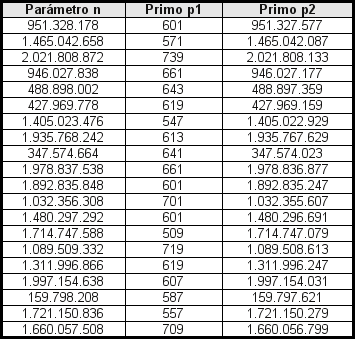
\includegraphics[width=0.5\textwidth]{Plots/Ej1-MayoresPrimos.png}
% \begin{center}
% Figura 1.2
% \end{center}
% \end{center}

Como se observa en la Figura 1.2, para los peores casos la diferencia entre cada uno de los primos soluci\'on es muy alta, muy cercana al par\'ametro de entrada $n$. Esto explica que la complejidad te\'orica no se corresponda con el tiempo de ejecuci\'on.

% \begin{center}
%  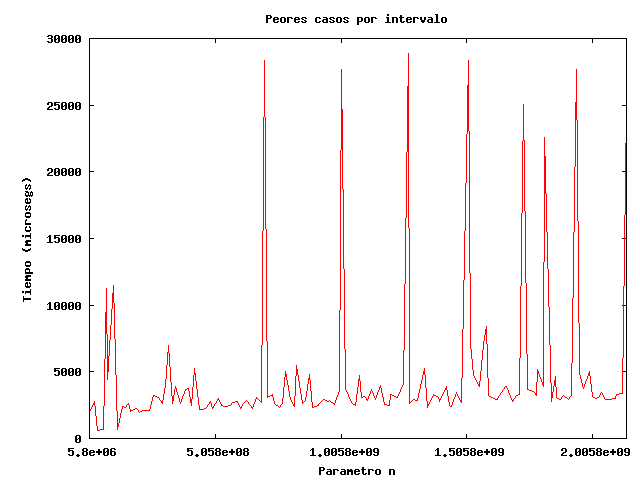
\includegraphics[width=0.7\textwidth]{Plots/Ej1-PeoresCasos.png}
% \begin{center}
% Figura 1.3
% \end{center}
% \end{center}

La idea de este gr\'afico es mostrar c\'uan irregular es el tiempo de ejecuci\'on del algoritmo. A pesar de haber hecho el esfuerzo de buscar los peores casos (mediante la aplicaci\'on de la Prueba 3), el tiempo que demoran los mismos difieren entre ellos considerablemente. Esto muestra que los peores casos no tienen una ralaci\'on directa con el tama\~{n}o de la entrada sino mas bien con la distribuci\'on desconocida de los n\'umeros primos pertenecientes al intervalo estudiado.

%TODO: explicacion de rand
%cita de casos patologicos
%mejores to do's

\section*{Conclusiones}

Este ejercicio nos mostr\'o un caso representativo en el que el tiempo de ejecuci\'on difiere notablemente a la complejidad calculada para el peor caso.

Para este algoritmo en particular se debe a que la funci\'on \textit{encontrarPrimos} alcanzar\'ia dicho peor caso si la conjetura de Goldbach fuese falsa, cuesti\'on que no sucede para ning\'un n\'umero que pueda tomar la func\'on (es decir, hasta el n\'umero mas grande almacenable en un \textit{int}). M\'as aun, esta demostrado que para n\'umeros mucho mas grandes que los testeados la conjetura se sigue cumpliendo (ver secci\'on Referencias para m\'as detalles) por lo que en el \'ambito cient\'ifico se cree que es cierta.

Tambi\'en vimos casos en los que entre n\'umeros cercanos tomados por la funci\'on, el tiempo de ejecuci\'on difiere considerablemente. Adem\'as notamos que a medida que el tama\~{n}o del par\'ametro de entrada crece el tiempo tamb\'ien lo hace, pero siempre muy lejos de los peores casos para dichas entradas. Estas situaciones se deben a la desconocida distribuci\'on de los n\'umeros primos entre los naturales, por lo que no podemos dar una explicaci\'on general que incluya todos los casos reales. Sin embargo, en base a todos los an\'alisis realizados, podemos concluir que para todos los casos computables por nuestro algoritmo el tiempo de ejecuci\'on ser\'a mas que aceptable.

\bigskip

\begin{center}
\section*{Ejercicio 2: Resoluci\'on de Puzzle}
\end{center}

\bigskip
\section*{Introducci\'on}

El objetivo del siguiente ejercicio es dise\~{n}ar un algoritmo que, dado un tablero de tama\~{n}o $n$ y $n^{2}$ fichas, determinar si existe una manera de colocar las fichas en el tablero, y en tal caso, retornarla. La condici\'on que determina si una ficha puede ser colocada es que, en cada uno de sus lados, contenga el mismo n\'umero que tiene la ficha con la que limita. Vale aclarar que las fichas no pueden ser rotadas y que los que lados limitan con un borde pueden tener cualquier n\'umero.

Cuando empezamos a pensar el ejercicio surgi\'o la soluci\'on trivial, tan simple como ineficiente, utilizando un algoritmo de fuerza bruta que prueba todas las permutaciones posibles de las fichas en el tablero. R\'apidamente se descart\'o esta opci\'on pues su costo es factorial. Se opt\'o entonces por aplicar la idea de \textit{backtracking} en la funci\'on, de esta manera, se toma una ficha del conjunto restante y se chequea si puede ser colocada en la pr\'oxima posici\'on. En caso afirmativo, la ficha se coloca en dicha posici\'on y se realiza el mismo procedimiento para la siguiente casilla del tablero, sino se sigue buscando hasta encontrar una ficha que pueda ser colocada. Si ninguna de las fichas restantes puede ser colocada en el tablero entonces se regresa a la posici\'on anterior (aqu\'i queda explicita la idea de \textit{backtracking}) y se prueba con otra. Por \'ultimo, se plante\'o el uso de diversas podas para mejorar el rendimiento del algoritmo. Se dejaron de lado distintas opciones, ya sea por dificultad de implementaci\'on o exceso de complejidad temporal o espacial, tomando finalmente la poda que mejor se ajust\'o a los requerimientos necesarios.

\section*{Algoritmo}

A continuaci\'on se presenta el pseudoc\'odigo del algoritmo para resolver el problema propuesto.

\begin{verbatim}
resolverPuzzle(fichas[0..n^2-1], n) 

  tablero[n][n]

  fichaActualEn[n][n]
  para i desde 0 hasta n-1
    para j desde 0 hasta n-1
      fichaActualEn[i][j] = 0

  fichasPuestas[0..n^2-1]
  para i desde 0 hasta n^2-1
    fichasPuestas[i] = false

  i = 0
  j = 0

  lista jardineroViejo = lista vacia
  lista jardineroNuevo = lista vacia
  metio = false
  volviolgunavez = false
  i_ant = 0
  j_ant = 0

  mientras i < n

    si !fichasPuestas[fichaActualEn[i][j]] 
    y encaja(fichas[fichaActualEn[i][j]], tablero, i, j)

      si i != n-1
        vaciar(jardineroNuevo)
        para k desde 0 hasta n^2-1
          si arriba(fichas[k]) = abajo(fichas[fichaActualEn[i][j]]) y !fichasPuestas[k]
            jardineroNuevo = jardineroNuevo U fichas[k]

      si j = 0 o i = n-1 o !puedoPodar(jardineroViejo, jardineroNuevo)

        si i != n-1
          jardineroViejo = jardineroNuevo

        tablero[i][j] = fichas[fichaActualEn[i][j]]
        fichasPuestas[fichaActualEn[i][j]] = true
        metio = true
        si j = n-1
          i = i + 1
          j = 0;
        sino
          j = j + 1

    si !metio

      volviolgunavez = false;
      mientras fichaActualEn[i][j] = n^2-1

        si i = 0 y j = 0
          devolver "No hay solucion"
        fichaActualEn[i][j] = 0
        si j = 0
          i = i - 1
          j = n-1
        sino
          j = j - 1

        fichasPuestas[fichaActualEn[i][j]] = false
        volviolgunavez = true

      si volviolgunavez = true
        si j = 0
          i_ant = i-1
          j_ant = n-1
        sino
          i_ant = i
          j_ant = j-1

        si (j_ant != 0 o i_ant != 0) y (i_ant != n-1)
          vaciar(jardineroViejo)
          para k desde 0 hasta n^2-1
            si arriba(fichas[k]) = abajo(fichas[fichaActualEn[i_ant][j_ant]]) 
            y !fichasPuestas[k]
              jardineroViejo = jardineroViejo U fichas[k]

      fichaActualEn[i][j] = fichaActualEn[i][j] + 1

  devolver tablero


puedoPodar(lista1, lista2)
  devolver interseccion(lista1, lista2) != vacio

encaja(ficha, tablero, i, j)
  (i = 0 o abajo(tablero[i-1][j]) = arriba(ficha)) y
  (j = 0 o derecha(tablero[i][j-1]) = izquierda(ficha))

\end{verbatim}

Antes de comenzar, para la implementaci\'on se utilizaron las siguientes estructuras:
\begin{itemize}
 \item \textbf{tablero:} es la matriz en donde se ir\'an colocando las fichas que son posible soluci\'on hasta un paso determinado. Fue implementada mediante un arreglo de arreglos.
\item \textbf{fichas:} es el arreglo que contiene todas las fichas de entrada del algoritmo (provenientes de Tp1Ej2.in).
\item \textbf{fichaActualEn:} cada posici\'on de esta matriz contiene la posici\'on en el arreglo fichas de la ficha actual (la ficha que est\'a siendo evaluada como soluci\'on del tablero en un paso del algoritmo) para cada una de las casillas del tablero. Al igual que tablero, esta estructura est\'a implementada con un arreglo de arreglos.
\item \textbf{fichasPuestas:} es un arreglo de datos \textit{booleanos} del mismo tama\~{n}o que fichas, que indica si una determinada ficha est\'a colocada en el tablero.
\item \textbf{jardineroViejo/Nuevo:} estructura implementada a trav\'es de una lista enlazada, que se utiliza, como veremos m\'as adelante, para aplicar las podas del algoritmo.
\end{itemize}

Luego de inicializar las estructuras, comienza el ciclo principal que intentar\'a colocar las fichas de una en una en el tablero finalizando una vez que este se complete (es decir, cuando $i = n$). En primer lugar se verifica que la ficha actual, apuntada por fichaActualEn[i][j], encaje en la posici\'on (i,j) del tablero y que la misma no pertenezca al conjunto de fichas puestas. En caso afirmativo, se procede a evaluar si se puede realizar una poda (posteriormente explicada en la secci\'on Poda). De no ser factible esta \'ultima, se coloca la ficha en el tablero y se avanza a la siguiente posici\'on del mismo. Si se llega a aplicar la poda, la ficha no se inserta.

En caso de que no se haya insertado una ficha en alg\'un paso del algoritmo, se intentar\'a colocar la siguiente ficha (es decir, se aumenta fichaActualEn[i][j]). Si la ficha revisada resulta ser la \'ultima por revisar, se retrocede hasta la posici\'on del tablero m\'as cercana que tenga fichas por revisar a\'un. Como se sugiri\'o anteriormente, dicha comprobaci\'on se realiza por medio de la matriz fichaActualEn. Si se intentara retroceder de la posici\'on inicial (0,0) la instancia recibida no tiene soluci\'on y, por lo tanto, el algoritmo finaliza informando tal evento.

\subsection*{Poda}

Con el fin de optimizar el rendimiento del algoritmo se aplicó el concepto de \textit{poda} visto en clase, relativo a todo algoritmo de \textit{backtracking}. La poda propuesta consiste en la siguiente idea que veremos a continuaci\'on. Cabe aclarar que esta poda no se aplica a los bordes izquierdo e inferior del tablero, ya que idea en cuesti\'on no es aplicable en dichas posici\'ones.

En primer lugar, cada vez que se desea añadir una ficha, se genera un conjunto determinado de fichas relacionadas a la misma que llamaremos ``jardinero''. Un ``jardinero`` est\'a conformado por todas las fichas que pueden unirse por debajo con la ficha a la cual est\'a asociada el jardinero. . Como se puede ver en el pseudoc\'odigo, una vez que se verific\'o que la ficha actual es candidata para ser insertada en el tablero (aquella que encaja en la posici\'on actual seg\'un lo visto antes) se crea el jardinero asociado a esa ficha que denominaremos \textit{jardineroNuevo}. En el caso de encontrarse en el borde izquierdo del tablero, la poda no se aplica y simplemente \textit{jardineroNuevo} pasa a ser \textit{jardineroViejo}. Este \'ultimo siempre va a ser el jardinero asociado a la ficha anterior a la posici\'on actual del tablero. 

Para los casos no pertenecientes al borde izquierdo (ni inferior), se evalua si se puede realizar la poda mediante la func\'ion \textit{puedoPodar(jardineroViejo, jardineroNuevo)}. Tal como muestra el pseudoc\'odigo, la misma verifica si hay intersecci\'on entre ambos jardineros, es decir, si alguna de las fichas de un jardinero puede encajar con alguna ficha del otro. Si ninguna encaja, implica que la ficha actual (\textit{fichas[fichaActualEn[i][j]]}) que se estaba por insertar no puede ir junto con la ficha anterior (ficha a su izquierda) en esa ubicaci\'on del tablero (quiz\'as si pueden formar parte del borde inferior). Observando este hecho desde el punto de vista de un algoritmo de \textit{backtracking}, al descartar esta posible soluci\'on se evita tener que ver todas las soluciones que involucren el haber insertado tal ficha en el tablero, evitando as\'i tener que analizar esa ''rama`` del \'arbol k-ario de posibles soluciones. Por este motivo, podemos afirmar que este procedimiento realizado constituye una \textit{poda} del \'arbol de \textit{backtracking}.

Para poder mantener el invariante de tener siempre un jardinero asociado a la ficha anterior a la actual (\textit{jardineroViejo}) es necesario contemplar el caso en el que se retrocede a posiciones anteriores del tablero y se retira fichas insertadas anteriormente. En tal caso, como se puede ver en el pseudoc\'odigo, se genera un \textit{jardineroViejo} que se asocia la posici\'on anterior a la actual (es decir, la posici\'on (i\_ant, j\_ant)). De este modo, al iterar nuevamente, el jardinero de la nueva ficha a insertar (jardineroNuevo) puede evaluarse con el jardineroViejo para ver si se puede realizar una nueva poda.

Como veremos enseguida, esta poda resulta efectiva en la pr\'actica, disminuyendo notoriamente los tiempos de ejecuci\'on.

\section*{Complejidad}

Como el algoritmo propuesto se basa en la t\'ecnica de \textit{backtracking}, la complejidad del mismo en el peor caso es similar a la de un algoritmo de fuerza bruta. En este tipo de algoritmos, se generan todas las soluciones posibles y se eval\'uan para determinar si cumplen con el problema a resolver. La complejidad de generar y revisar todas las soluciones posibles es exponencial y, en particular, el algoritmo de fuerza bruta aplicado al problema presentado ser\'ia $O(n!)$, con $n$ la cantidad de fichas del tablero. A pesar de que los algoritmos de \textit{backtracking} descartan gran cantidad de casos y aplican podas para reducir el tiempo de ejecuci\'on, existen casos patol\'ogicos en que pocas de estas optimizaciones pueden ser utilizadas y, por lo tanto, se recorran todas las ramas de soluciones. Estos casos hacen que la complejidad en el peor caso del algoritmo presentado sea la misma que la de un algoritmo de fuerza bruta, es decir $O(n!)$ (siendo $n$ la cantidad de fichas totales del tablero). Sin embargo, como estudiaremos en posteriores secciones, el tiempo de ejecuci\'on del algoritmo difiere significativamente del tiempo del algoritmo de fuerza bruta.

\section*{An\'alisis de resultados}

En la siguiente secci\'on se mostrar\'an los an\'alisis realizados para tableros de distinto tama\~{n}o. El enfoque principal de las pruebas radica en estudiar los tiempos de ejecuci\'on del algoritmo con y sin la poda. Para esto se implement\'o un algoritmo que genera tableros aleatorios de un tama\~{n}o $n$ pasado como par\'ametro. De esta manera, utilizando dicho algoritmo para distintos valores de $n$, se contrastaron ambos metodos (con y sin poda) con la cota estudiada ($n!$) arrojando los siguientes resultados. Vale aclarar que se utiliz\'o una escala logar\'itmica sobre el eje de ordenadas ya que los tiempos de ejecuci\'on toman valores muy altos, adem\'as, para realizar los gr\'aficos expuestos, se utilizaron tableros hasta un tama\~{n}o de $n=15$ pues para mayores valores los tiempos son excesivos.

% \begin{center}
%  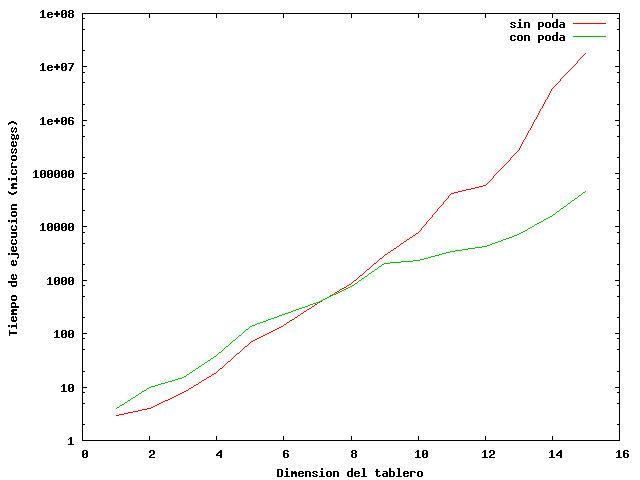
\includegraphics[width=0.7\textwidth]{Plots/Ej2-Complejidad2.png}
% \begin{center}
% Figura 2.1
% \end{center}
% \end{center}
% 
% \begin{center}
%  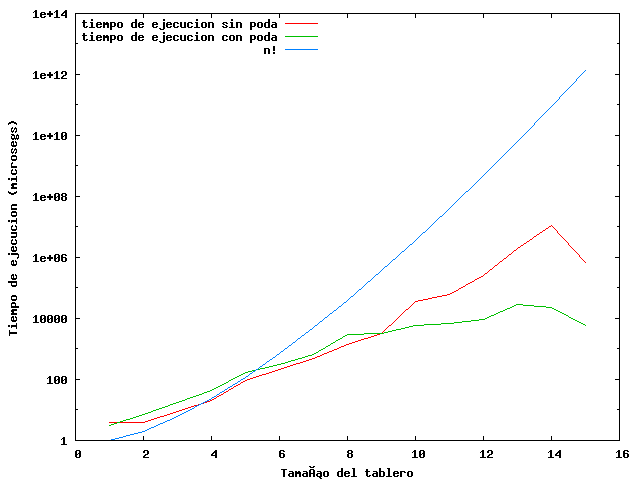
\includegraphics[width=0.7\textwidth]{Plots/Ej2-Complejidad1.png}
% \begin{center}
% Figura 2.2
% \end{center}
% \end{center}

Como se puede apreciar en ambos gr\'aficos, los tiempos de ejecuci\'on de los dos algoritmos son sensiblemente menores que los de la complejidad teorica calculada para el peor caso ($O(n!)$). Esto concuerda con lo esperado ya que como se dijo en anteriores secciones, salvo en casos patol\'ogicos, en la pr\'actica el metodo de \textit{backtracking} aplicado a este problema es mucho m\'as eficiente.

Con respecto a las diferentes resultados obtenidos con los dos m\'etodos, vemos reflejado que efectivamente la poda produce una importante mejora en el rendimiento. Si bien para tableros peque\~{n}os el rendimiento es similar (es m\'as, en la mayor\'ia de los casos para $n$ chicos el m\'etodo que utiliza la poda suele ser menos eficaz), esto no es de importancia ya que en dichos casos, al no manejar gran cantidad de datos, el tiempo de ejecuci\'on no alcanza valores muy altos. Por el contrario, cuando tomamos valores de $n$ mas grandes (aprox $n\geq10$), se puede apreciar que la poda descarta gran cantidad de soluciones no posibles, lo que incide directamente en la eficiencia de la aplicaci\'on. De hecho, cuando se analizaron tableros de tama\~{n}o mayor que 15, el tiempo que llev\'o a cabo el algoritmo sin la poda para buscar una soluci\'on result\'o excesivo, situaci\'on que no ocurre cuando se utiliza la poda para tableros de hasta $n=25$.

Por \'ultimo, cabe notar que el tiempo de ejecuci\'on real no est\'a estrictamente relacionado con el tama\~{n}o de entrada. Podemos apreciarlo en la \textit{Figura 2.2}, donde la ejecuci\'on de el algoritmo con y sin la poda tom\'o m\'as tiempo para $n=14$ que para $n=15$. Esto se debe a que, adem\'as de depender de la dimensi\'on del tablero, la eficiencia del algoritmo estar\'a relacionada con la distribuci\'on de las fichas recibidas.

\section*{Conclusiones}

A lo largo del desarrollo del ejercicio, se experimentaron las particularidades de un algoritmo de \textit{backtracking}. Nos encontramos con diversas dificultades en la implementaci\'on, a pesar de que la idea intuitiva del algoritmo es relativamente simple. Adem\'as, llegamos a la conclusi\'on de que, si bien la complejidad en peor caso es muy elevada, el algoritmo en general suele ser mucho m\'as eficiente que algoritmos que utilizan la t\'ecnica de fuerza bruta para resolver este tipo de problemas. 

Los principales incovenientes que surgen al implementar un algoritmo de \textit{backtracking} tienen que ver con la elecci\'on de la poda. Al momento de dicha elecci\'on, se deben considerar los aspectos de eficiencia, dificultad en la implementaci\'on y sobre todo, los beneficios (en relaci\'on al tiempo de ejecuci\'on) que esta provocar\'ia. Al pensar en detalle cada uno de las posibles podas, estos factores fueron determinantes para tomar una decisi\'on; podas que parec\'ian muy eficientes en principio, resultaban muy dif\'iciles de implementar y no aportaban cambios significativos que justifiquen su uso. A su vez, podas que parec\'ian descartar muchos casos, terminaban empeorando el tiempo de ejecuci\'on.

Es importante destacar que al aplicar la poda propuesta, el algoritmo mejora considerablemente en promedio. Esta situaci\'on resultaba esperable y pudo ser comprobada emp\'iricamente en las pruebas realizadas. Tambi\'en, se not\'o una relaci\'on entre la distribuci\'on de fichas de entrada y el tiempo de ejecuci\'on del algoritmo presentado. Por ejemplo, existen casos en los que la disposici\'on de las fichas no permitan hacer podas y otros en los que no sea necesario tener que reemplazar alguna ficha.

En conclusi\'on, la eficiencia del algoritmo de \textit{backtracking} depende fuertemente de las podas que se realicen y de la distribuci\'on probabil\'istica de los par\'ametros de entrada para casos promedio. Por esta raz\'on, la implementaci\'on de podas es determinante y justifica el tiempo invertido en idear las mismas.

\begin{center}
\section*{Ejercicio 3: C\'alculo de la mediana entre dos vectores}
\end{center}

\bigskip
\section*{Introducci\'on}

El problema que plantea este ejercicio es calcular la mediana entre dos vectores de n\'umeros enteros, es decir, el elemento que, una vez concatenados y ordenados los vectores, deja a ambos lados la misma cantidad de elementos. Seg\'un lo especificado en el problema, ambos vectores tienen la misma longitud y est\'an ordenados.

En principio, la soluci\'on trivial del problema fue descartada ya que el costo de realizarla era excesivo para los fines del ejercicio. Esta soluci\'on consist\'ia en concatenar ambos vectores, ordenarlos y posteriormente obtener la mediana a partir del elemento medio de dicha secuencia.

Descartada esta opci\'on, surgi\'o la idea de desechar una gran cantidad de elementos, cuando sea posible, para poder realizar los c\'alculos sobre una cantidad de n\'umeros considerablemente inferior a la inicial. De esta manera, la complejidad resultar\'ia del costo de descartar los elementos apropiados y luego hacer el c\'alculo con una cantidad peque\~{n}a de elementos. Evidentemente, nuestro algoritmo seguir\'ia el concepto de Divide and Conquer cl\'asico.

Con las ideas m\'as claras, notamos que descartando la misma cantidad de elementos mayores o iguales a la mediana, que menores o iguales a ella, \'esta se manten\'ia como valor medio de los vectores generados a partir de los elementos no descartados. R\'apidamente, nos dimos cuenta que la mediana de concatenar dos vectores ordenados, se encuentra entre los elementos mayores a la mediana del vector con menor valor medio y los elementos menores a la mediana del vector con mayor valor medio (conjetura que luego se demostrar\'a).

Planteado todo esto, result\'o sencillo escribir el pseudoc\'odigo de nuestro algoritmo. 

\section*{Algoritmo}

A continuaci\'on se mostrar\'a el pseudoc\'odigo del algoritmo implementado seguido de una demostraci\'on de su correctitud.

\begin{verbatim}
medianaRecursiva (vector x[0..n-1], vector y[0..n-1])

  si n == 1
    si x[0] > y[0]
      devolver y[0]
    sino
      devolver x[0]

  si n == 2
    si x[0] == y[0]
      devolver x[0]
    si x[0] > y[0]
      si x[0] > y[1]
        devolver y[1]
      sino
        devolver x[0]
    sino
      si x[1] > y[0]
        devolver y[0]
      sino
        devolver x[1]

  si n > 2
    si n es impar
      medio = n / 2
    sino
      medio = n / 2 - 1;
    si x[medio] > y[n/2]
      devolver medianaRecursiva(x[0..medio], y[n/2..n-1]);
    sino
      devolver medianaRecursiva(x[medio..n-1], y[0..n/2]);
\end{verbatim}

Con respecto a la implementaci\'on del algoritmo, la misma result\'o bastante sencilla de realizar en el lenguaje C++, utilizando las operaciones b\'asicas que provee el lenguaje y usando arreglos b\'asicos para la reprentaci\'on de los vectores. La \'unica parte no trivial radica en el uso de punteros para lograr llamar recursivamente a la func\'on con las ``mitades'' correspondientes de cada arreglo. Tambi\'en, cabe notar que en la implementaci\'on fue necesario pasar como par\'ametro extra el tama\~{n}o de los arreglos que reprentan a los vectores por cuestiones intr\'insicas al manejo de arreglos din\'amicos en C++.

Como se puede apreciar, el algoritmo sigue los pasos de un algoritmo cl\'asico de \textit{divide and conquer} dividiendo el problema en arreglos de menor tama\~{n}o al ir descartando elementos mayores y menores a la mediana. De esta manera, si logramos mostrar que en cada llamado recursivo la mediana original es la misma que la de los dos nuevos arreglos, entonces podremos asegurar que el algoritmo es correcto. Para mostrar esto primero veremos que en cada paso la mediana sigue estando dentro de alguno de los arreglos, y luego que los n\'umeros menores o iguales a la mediana descartados son la misma cantidad que los n\'umeros mayores o iguales a la misma que se descartan.

\subsection*{Demostraci\'on de que la mediana se encuentra en el pr\'oximo llamado recursivo}

Dividiremos la demostraci\'on en dos casos, cuando la longitud de los arreglos iniciales es impar y cuando es par.

Sean $X$ e $Y$ los arreglos iniciales, entonces si llamo $A$ a $concatenar(X,Y)$ tengo que $ordenar(A)=[a_{1},a_{2},..,a_{n},..,a_{2n}]$, como la longitud de $A$ es par, su mediana es $a_{n}$. Se puede ver entonces que la mediana tiene $n-1$ elementos menores o iguales a ella ($A[1..n-1]$) y n elementos mayores o iguales ($A[n+1..2n]$).

\begin{enumerate}
 \item Longitud impar:
  
Los arreglos que tomar\'a la funci\'on para el llamado recursivo estan dados por la comparaci\'on entre las medianas de los mismos siendo $x_{(n+1)/2}$ la mediana de $X$ e $y_{(n+1)/2}$ la mediana de $Y$.
\begin{enumerate}
\item $x_{(n+1)/2}\geq y_{(n+1)/2}$:

En este caso el algoritmo toma como nuevos arreglos a $X[1..(n+1)/2]$ e $Y[(n+1)/2..n]$. Supongo ahora, que $m$ (a partir de ahora nos referiremos asi a la mediana) no est\'a en los nuevos arreglos, es decir, pertenece a $X((n+1)/2..n]$ o a $Y[1..(n+1)/2)$.
\begin{enumerate}
\item
 Si $m \in X((n+1)/2..n] \Longrightarrow m \geq x_{(n+1)/2}$. Si $m=x_{(n+1)/2}$ entonces SI pertenece a los nuevos arreglos pues $x_{(n+1)/2}$ pertenece. Si no son iguales entonces $m>x_{(n+1)/2} \Longrightarrow m>x \,\,\forall x \in X[1..(n+1)/2]$. Ademas si $m>x_{(n+1)/2}\geq y_{(n+1)/2} \Longrightarrow m>y \,\,\forall y \in Y[1..(n+1)/2]$. Como $X[1..(n+1)/2]$ y $Y[1..(n+1)/2]$ tienen $(n+1)/2$ elementos cada uno entonces $m$ es mayor a $2((n+1)/2)=n+1$ elementos lo que es absurdo porque la mediana solo puede tener tener $n-1$ elementos menores por lo visto anteriormente.
\item
 Si $m \in Y[1..(n+1)/2) \Longrightarrow m \leq y_{(n+1)/2}$. Si $m=y_{(n+1)/2}$ entonces SI pertenece a los nuevos arreglos pues $y_{(n+1)/2}$ pertenece. Si no son iguales entonces $m<y_{(n+1)/2} \Longrightarrow m<y \,\,\forall y \in Y[(n+1)/2..n]$. Ademas si $m<y_{(n+1)/2}\leq x_{(n+1)/2} \Longrightarrow m<x \,\,\forall x \in X[(n+1)/2..n]$. Como $X[(n+1)/2..n]$ y $Y[(n+1)/2..n]$ tienen $(n+1)/2$ elementos cada uno entonces $m$ es menor a $2((n+1)/2)=n+1$ elementos lo que es absurdo porque la mediana solo puede tener tener $n$ elementos mayores por lo visto anteriormente.
\end{enumerate}

De esta manera queda demostrado que si $n$ es impar y $x_{(n+1)/2}\geq y_{(n+1)/2}$ entonces la mediana pertenece a alguno de los nuevos arreglos pasados como par\'ametro.

\item $x_{(n+1)/2}<y_{(n+1)/2}$:

En este caso el algoritmo toma como nuevos arreglos a $X[(n+1)/2..n]$ e $Y[1..(n+1)/2]$. Supongo ahora, que $m$ no est\'a en los nuevos arreglos, es decir, pertenece a $X[1..(n+1)/2)$ o a $Y((n+1)/2..n]$. 
\begin{enumerate}
\item
 Si $m \in X[1..(n+1)/2) \Longrightarrow m \leq x_{(n+1)/2}$. Si $m=x_{(n+1)/2}$ entonces SI pertenece a los nuevos arreglos pues $x_{(n+1)/2}$ pertenece. Si no son iguales entonces $m<x_{(n+1)/2} \Longrightarrow m<x \,\,\forall x \in X[(n+1)/2..n]$. Ademas si $m<x_{(n+1)/2}< y_{(n+1)/2} \Longrightarrow m<y \,\,\forall y \in Y[(n+1)/2..n]$. Como $X[(n+1)/2..n]$ y $Y[(n+1)/2..n]$ tienen $(n+1)/2$ elementos cada uno entonces $m$ es menor a $2((n+1)/2)=n+1$ elementos lo que es absurdo porque la mediana solo puede tener tener $n-1$ elementos menores por lo visto anteriormente.
\item
 Si $m \in Y((n+1)/2..n] \Longrightarrow m \geq y_{(n+1)/2}$. Si $m=y_{(n+1)/2}$ entonces SI pertenece a los nuevos arreglos pues $y_{(n+1)/2}$ pertenece. Si no son iguales entonces $m>y_{(n+1)/2} \Longrightarrow m>y \,\,\forall y \in Y[1..(n+1)/2]$. Ademas si $m>y_{(n+1)/2}> x_{(n+1)/2} \Longrightarrow m>x \,\,\forall x \in X[1..(n+1)/2]$. Como $X[(n+1)/2..n]$ y $Y[(n+1)/2..n]$ tienen $(n+1)/2$ elementos cada uno entonces $m$ es mayor a $2((n+1)/2)=n+1$ elementos lo que es absurdo porque la mediana solo puede tener tener $n$ elementos mayores por lo visto anteriormente.
\end{enumerate}

De esta manera queda demostrado que si $n$ es impar y $x_{(n+1)/2}\geq y_{(n+1)/2}$ entonces la mediana pertenece a alguno de los nuevos arreglos pasados como par\'ametro.
\end{enumerate}

\item Longitud par

Los arreglos que tomar\'a la funci\'on para el llamado recursivo estan dados por la comparaci\'on entre $x_{n/2}$ e $y_{n/2+1}$.
\begin{enumerate}
\item $x_{n/2}\geq y_{n/2+1}$:
En este caso el algoritmo toma como nuevos arreglos a $X[1..n/2]$ e $Y[n/2+1..n]$. Supongo ahora, que $m$ no est\'a en los nuevos arreglos, es decir, pertenece a $X(n/2..n]$ o a $Y[1..n/2+1)$. 
\begin{enumerate}
\item
 Si $m \in X(n/2..n] \Longrightarrow m \geq x_{n/2}$. Si $m=x_{n/2}$ entonces SI pertenece a los nuevos arreglos pues $x_{n/2}$ pertenece. Si no son iguales entonces $m>x_{n/2} \Longrightarrow m>x \,\,\forall x \in X[1..n/2]$. Ademas si $m>x_{n/2}\geq y_{n/2+1} \Longrightarrow m>y \,\,\forall y \in Y[1..n/2+1]$. Como $X[1..n/2]$ y $Y[1..n/2+1]$ tienen $n/2$ y $n/2+1$ elementos respectivamente entonces $m$ es mayor a $n/2+n/2+1=n+1$ elementos lo que es absurdo porque la mediana solo puede tener tener $n-1$ elementos menores por lo visto anteriormente.
\item
  Si $m \in Y[1..n/2+1) \Longrightarrow m \leq y_{n/2+1}$. Si $m=y_{n/2+1}$ entonces SI pertenece a los nuevos arreglos pues $y_{n/2+1}$ pertenece. Si no son iguales entonces $m<y_{n/2+1} \Longrightarrow m<y \,\,\forall y \in Y[n/2+1..n]$. Ademas si $m<y_{n/2+1}\leq x_{n/2} \Longrightarrow m<x \,\,\forall x \in X[n/2..n]$. Como $X[n/2..n]$ y $Y[n/2+1..n]$ tienen $n/2+1$ y $n/2$ elementos respectivamente entonces $m$ es menor a $n/2+1+n/2=n+1$ elementos lo que es absurdo porque la mediana solo puede tener tener $n$ elementos mayores por lo visto anteriormente.
\end{enumerate}

De esta manera queda demostrado que si $n$ es par y $x_{n/2}\geq y_{n/2+1}$ entonces la mediana pertenece a alguno de los nuevos arreglos pasados como par\'ametro.


\item $x_{n/2}<y_{n/2+1}$:
En este caso el algoritmo toma como nuevos arreglos a $X[n/2..n]$ e $Y[1..n/2+1]$. Supongo ahora, que $m$ no est\'a en los nuevos arreglos, es decir, pertenece a $X[1..n/2)$ o a $Y(n/2+1..n]$. 
\begin{enumerate}
\item
 Si $m \in X[1..n/2) \Longrightarrow m \leq x_{n/2}$. Si $m=x_{n/2}$ entonces SI pertenece a los nuevos arreglos pues $x_{n/2}$ pertenece. Si no son iguales entonces $m<x_{n/2} \Longrightarrow m<x \,\,\forall x \in X[n/2..n]$. Ademas si $m<x_{n/2}\leq y_{n/2+1} \Longrightarrow m<y \,\,\forall y \in Y[n/2+1..n]$. Como $X[n/2..n]$ y $Y[n/2+1..n]$ tienen $n/2+1$ y $n/2$ elementos respectivamente entonces $m$ es menor a $n/2+1+n/2=n+1$ elementos lo que es absurdo porque la mediana solo puede tener tener $n$ elementos mayores por lo visto anteriormente.
\item
  Si $m \in Y(n/2+1..n]\Longrightarrow m \geq y_{n/2+1}$. Si $m=y_{n/2+1}$ entonces SI pertenece a los nuevos arreglos pues $y_{n/2+1}$ pertenece. Si no son iguales entonces $m>y_{n/2+1} \Longrightarrow m>y \,\,\forall y \in Y[1..n/2+1]$. Ademas si $m>y_{n/2+1}> x_{n/2} \Longrightarrow m>x \,\,\forall x \in X[1..n/2]$. Como $X[1..n/2]$ y $Y[1..n/2+1]$ tienen $n/2$ y $n/2+1$ elementos respectivamente entonces $m$ es mayor a $n/2+n/2+1=n+1$ elementos lo que es absurdo porque la mediana solo puede tener tener $n-1$ elementos menores por lo visto anteriormente.
\end{enumerate}

De esta manera queda demostrado que si $n$ es par y $x_{n/2}\geq y_{n/2+1}$ entonces la mediana pertenece a alguno de los nuevos arreglos pasados como par\'ametro.

\end{enumerate}

\end{enumerate}

En conclusi\'on queda demostrado que siempre que se realiza un llamado recursivo, la mediana pertenece a uno de los dos arreglos pasados como par\'ametro.


\subsection*{Demostraci\'on de que se descartan la misma cantidad de elementos mayores o iguales y menores o iguales que la mediana}

Sean $X$ e $Y$ los arreglos pasados como par\'ametro y $n$ su longituud.

\begin{enumerate}\item
Si la longitud de los arreglos es impar, los elemenos que se descartan dependen de la comparaci\'on entre $x_{(n+1)/2}$ e $y_{(n+1)/2}$.
\begin{enumerate}
\item
Si $x_{(n+1)/2} \geq y_{(n+1)/2}$ entonces se descarta $X((n+1)/2..n]$ e $Y[1..(n+1)/2)$. Como la mediana es menor o igual que $x_{(n+1)/2}$ por estar inclu\'ida y los elementos de $X((n+1)/2..n]$ son mayores o iguales que $x_{(n+1)/2}$ entonces se descartan $(n-1)/2$ elementos mayores o iguales que la mediana. Ademas como la mediana es mayor o igual que $y_{(n+1)/2}$ por estar inclu\'ida y los elementos de $Y(1..(n+1)/2]$ son menores o iguales que $y_{(n+1)/2}$ entonces se descartan $(n-1)/2$ elementos menores o iguales que la mediana. De esta manera queda demostrado que para el caso en que n es impar y $x_{(n+1)/2}$ es mayor o igual a $y_{(n+1)/2}$ se descartan la misma cantidad de elementos menores o igual que mayores o iguales que la mediana.

\item
Si $x_{(n+1)/2} < y_{(n+1)/2}$ entonces se descarta $Y((n+1)/2..n]$ e $X[1..(n+1)/2)$. Como la mediana es mayor o igual que $x_{(n+1)/2}$ por estar inclu\'ida y los elementos de $X[1..(n+1)/2)$ son menores o iguales que $x_{(n+1)/2}$ entonces se descartan $(n-1)/2$ elementos menores o iguales que la mediana. Ademas como la mediana es menor o igual que $y_{(n+1)/2}$ por estar inclu\'ida y los elementos de $Y((n+1)/2..n]$ son mayores o iguales que $y_{(n+1)/2}$ entonces se descartan $(n-1)/2$ elementos mayores o iguales que la mediana. De esta manera queda demostrado que para el caso en que n es impar y $x_{(n+1)/2}$ es menor o igual a $y_{(n+1)/2}$ se descartan la misma cantidad de elementos menores o igual que mayores o iguales que la mediana.
\end{enumerate}

\item
Si la longitud de los arreglos es par, los elementos que se descartan dependen de la comparaci\'on entre $x_{n/2}$ e $y_{n/2+1}$.  

\begin{enumerate}
\item
Si $x_{n/2} \geq y_{n/2+1}$ entonces se descarta $X(n/2..n]$ e $Y[1..n/2+1)$. Como la mediana es menor o igual que $x_{n/2}$ por estar inclu\'ida y los elementos de $X(n/2..n]$ son mayores o iguales que $x_{n/2}$ entonces se descartan $n/2$ elementos mayores o iguales que la mediana. Ademas como la mediana es mayor o igual que $y_{n/2+1}$ por estar inclu\'ida y los elementos de $Y[1..n/2+1)$ son menores o iguales que $y_{n/2+1}$ entonces se descartan $n/2$ elementos menores o iguales que la mediana. De esta manera queda demostrado que para el caso en que n es par y $x_{n/2}$ es mayor o igual a $y_{n/2+1}$ se descartan la misma cantidad de elementos menores o igual que mayores o iguales que la mediana.

\item
Si $x_{n/2} < y_{n/2+1}$ entonces se descarta $Y(n/2+1..n]$ e $X[1..n/2)$. Como la mediana es menor que $x_{n/2}$ por estar inclu\'ida y los elementos de $X[1..n/2)$ son mayores que $x_{n/2}$ entonces se descartan $n/2-1$ elementos menores o iguales que la mediana. Ademas como la mediana es mayor o igual que $y_{n/2+}$ por estar inclu\'ida y los elementos de $Y(n/2+1..n]$ son mayores o iguales que $y_{n/2+1}$ entonces se descartan $n/2-1$ elementos mayores o iguales que la mediana. De esta manera queda demostrado que para el caso en que n es par y $x_{n/2}$ es menor o igual a $y_{n/2+1}$ se descartan la misma cantidad de elementos menores o igual que mayores o iguales que la mediana.
\end{enumerate}

\end{enumerate}

Finalmente queda demostrado que en todos los casos se descartan la misma cantidad de elementos mayores o iguales y menores o iguales que la mediana.

Juntando ambas demostraciones podemos afirmar que en cada llamado recursivo la mediana original es la misma que la mediana entre la concatenaci\'on de los dos nuevos arreglos. Debido a esto, al aplicar sucesivos llamados a la funci\'on se desembocara en un caso base el cual nos devolver\'a el resultado buscado.

\section*{Complejidad}
 
En la presente secci\'on se calcular\'a la complejidad en el peor caso del algoritmo presentado bas\'andose en el modelo de c\'omputo uniforme.

La funci\'on presenta dos casos base que se dan cuando $n$ (variable que indica la longitud de los arreglos) toma los valores 1 \'o 2. En ambos casos el algoritmo s\'olo realiza comparaciones entre elementos y retorna un resultado, sin entrar en ning\'un ciclo.

Si n es mayor a 2 primero se realizan asignaciones y operaciones simples (tiempo constante) para luego efectuar un llamado recursivo. En el caso en que el tama\~{n}o de los arreglos es par, se toma $n=n/2$ como nuevo par\'ametro de longitud. En el caso impar, la longitud de los arreglos ser\'a $(n+1)/2$. De esta manera, cuando n es potencia de 2, el algoritmo ejecuta $\log(n)$ llamados recursivos hasta llegar a un caso base. De lo contrario se producen $\log(n)+1$ llamadas (se refiere a la parte entera de $\log(n)$).

Por lo tanto la funci\'on que determina la complejidad es:

$$T(n)=c+T(n/2)=c+c+T(n/4)=..= \sum_{i=1}^{\log(n)+1}c=c\sum_{i=1}^{\log(n)+1}1=c(\log(n)+1)$$
$$\Longrightarrow T(n)\in O(\log(n))$$

Por \'ultimo se estudiar\'a la complejidad en relaci\'on al tama\~{n}o de la entrada. Sea $t$ el tama\~{n}o de la entrada, $X$ e $Y$ los arreglos pasados como par\'ametro y $n$ su tama\~{n}o.

$$t=\log(n)+\sum_{i=1}^{n}\log(X_{i})+\sum_{i=1}^{n}\log(Y_{i})>\log(n)+\sum_{i=1}^{n} 1+\sum_{i=1}^{n} 1$$
$$=\log(n)+2n>\log(n)$$
\hspace*{90pt}$\Longrightarrow$ como $T(n)\in O(\log(n))$ y $\log(n)<t$ $\Longrightarrow T(t)\in O(t)$

\section*{An\'alisis de resultados}

Con el prop\'osito de analizar la eficiencia del algoritmo propuesto se construy\'o una simple aplicaci\'on de prueba (ver pseudoc\'odigo debajo) que calcula el tiempo de ejecucion de la funci\'on \textit{medianaRecursiva} para vectores aleatorios de tama\~{n}o variable entre $2$ y $2*10^{8}$. En principio, las pruebas realizadas difer\'ian de las mencionadas anteriormente, ya que el tama\~{n}o de las instancias probadas era mucho menor (entre $1$ y $10^{4}$). Sin embargo, como se ver\'a m\'as adelante, los resultados para este tipo de pruebas no reflejaba datos significativos para el an\'alisis del algoritmo y su complejidad.

\begin{verbatim}
para i desde 2 hasta 2*10^8
	vector x[1..i]
	vector y[1..i]

	x[1] = numero aleatorio entre 0 y 20
	y[1] = numero aleatorio entre 0 y 20
	
	para j desde 2 hasta i
		x[j] = x[j-1] + numero aleatorio entre 0 y 20
		y[j] = y[j-1] + numero aleatorio entre 0 y 20

	T = tiempo que tarda la funcion medianaRecursiva(x,y,i) en microsegundos

	guardar en Ej3-Complejidad.txt la linea "i T"
	i = i*2
\end{verbatim}

A continuaci\'on se presentan los resultados de la prueba realizada.

% \begin{center}
%  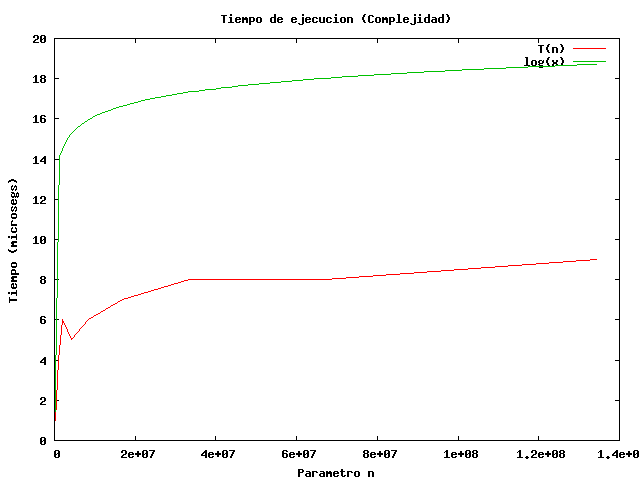
\includegraphics[width=0.7\textwidth]{Plots/Ej3-Complejidad.png}
% \begin{center}
% Figura 3.1
% \end{center}
% \end{center}

Como se puede observar en el gr\'afico, los tiempos de ejecuci\'on del algoritmo son muy bajos en relaci\'on al tama\~{n}o de la entrada. Esta fue la raz\'on por la que se descart\'o probar s\'olo casos peque\~{n}os para verificar la eficiencia del algoritmo y se opt\'o por analizar casos en el que el tama\~{n}o de la entrada creciera exponencialmente. A simple vista se puede observar que el gr\'afico de la funci\'on que mide el tiempo tiene el mismo comportamiento que la funci\'on de complejidad te\'orica. De este modo, adem\'as de la demostraci\'on te\'orica de la complejidad, se obtiene una prueba emp\'irica de que esta misma es correcta.

\section*{Conclusiones}

Este ejercicio nos hizo utilizar la t\'cnica de Divide and Conquer y nos mostr\'o varias de sus caracter\'isticas. La necesidad de utilizar 
esta t\'ecnica result\'o de la b\'usqueda de disminuir la complejidad lineal propuesta por la solución trivial.
	La complejidad obtenida muestra la relaci\'on que hay en ciertos algoritmos Divide and Conquer, entre el costo temporal de resolverlo 
y la cantidad de elementos de entrada. En este caso ni siquiera fue necesario leer cada uno de los elementos gracias a que cont\'abamos con
el orden de los vectores.
	En nuestro algoritmo el costo de cada una de las divisiones y cada una de las conquistas es contante, permitiendo que s\'olo 
la cantidad de llamadas a problemas m\'as peque\~{n}os defina la complejidad. Esta propiedad no logra s\'olo ser eficiente, sino que adem\'as, 
permite un c\'alculo sencillo de la complejidad temporal. En las pruebas emp\'iricas realizadas, puede observarse como el tiempo que toma realizar nuestro algoritmo,
es notablemente inferior al del tama\~{n}o de la entrada. Cabe destacar que nuestro algoritmo hace una cantidad similar de operaciones en todos los casos (para un mismo
tama\~{n}o de la entrada), ya que para calcular la mediana siempre debe llegar al caso base. Esto ayuda a la demostraci\'on de la correctitud del algortimo y lo hace 
m\'as natural. Puede observarse en el gr\'afico de nuestras pruebas, la ausencia de grandes picos, que muestra emp\'iricamente que para entradas de similar tama\~{n}o, el 
tiempo demandado ser\'a similar .
	Realizar este ejercicio tambi\'en nos mostr\'o la sencillez y la naturalidad con la que se pueden implementar los algoritmos divide and conquer mediante un 
m\'etodo recursivo, aunque claro, esto puede cambiar dependiendo de lo complejo que sea implementar la divisi\'on y la conquista. 
	En definitiva, se puede concluir que en ciertos casos,y en este en particular, los algoritmos Divide and Conquer son f\'aciles de implementar, eficientes en el peor caso, y es 
sencillo calcular su complejidad.


\end{document}